The user begins by using \karma's existing capability to model the artists in the CSV file as crm:E21\_Person in an \rtworml mapping shown in Figure~\ref{fig:simple-model-screenshot}.  
\karma can use this mapping to generate RDF,  
and can also compare it to retrieve other mappings, discovering new related sources that can be integrated with the artist dataset.
\begin{figure*}[b]
\centering
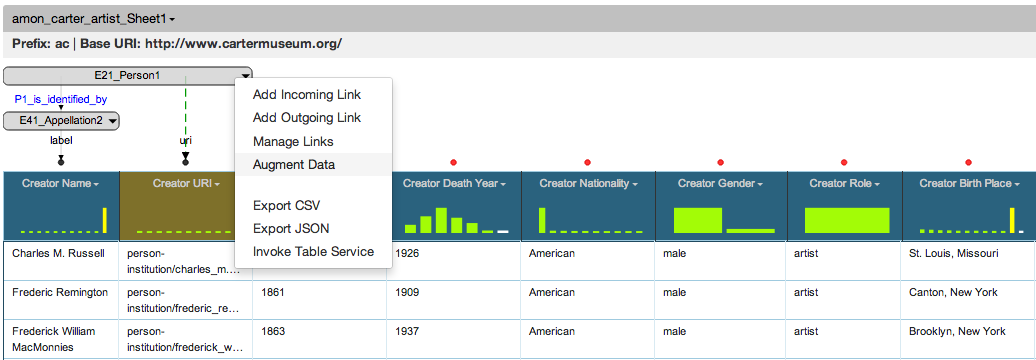
\includegraphics[width=4.8in]{images/4-simple-model.png}
\vspace{-20pt}
\caption{A \karma user creates an \rtworml mapping for a CSV file of a museum's artists' biographical records and clicks 'Augment Data' to discover new data sources}
\vspace{-21pt}
\label{fig:simple-model-screenshot}
\end{figure*}